\documentclass[12pt, a4paper]{article}
\usepackage[utf8]{inputenc}
\usepackage{amsmath}
\usepackage{amsthm}
\usepackage{amssymb}
\usepackage{graphicx}
\usepackage{parskip}
\usepackage{hyperref}
\usepackage{fancyhdr}
\usepackage{lastpage}
\usepackage[vlined,ruled]{algorithm2e}
\usepackage[acronym]{glossaries}
\usepackage{caption}
\usepackage{titlesec}
\usepackage{tikz}
\usetikzlibrary{arrows,automata}

\titleformat{\section}
  {\normalfont\bfseries}{Problem 5.\thesection}
  {0em}{}

\titleformat{\subsection}
  {\normalfont\bfseries}{5.\thesubsection}
  {0em}{}

\titleformat{\subsubsection}
  {\normalfont\bfseries}{5.\thesubsection}
  {0em}{}

\title{%
  Stochastic Network Modeling \\
  Homework 5 - Solutions
}
\author{%
  Juan Pablo Royo Sales\\
  \small{Universitat Politècnica de Catalunya}
}
\date\today

\pagestyle{fancy}
\fancyhf{}
\fancyhead[C]{}
\fancyhead[R]{Juan Pablo Royo Sales - UPC MIRI}
\fancyhead[L]{SNM - Homework 5}
\fancyfoot[L,C]{}
\fancyfoot[R]{Page \thepage{} of \pageref{LastPage}}
\setlength{\headheight}{15pt}
\renewcommand{\headrulewidth}{0.4pt}
\renewcommand{\footrulewidth}{0.4pt}

\renewcommand{\qedsymbol}{$\blacksquare$}

\begin{document}

\maketitle

\section{}
\subsection{}
\subsection{}
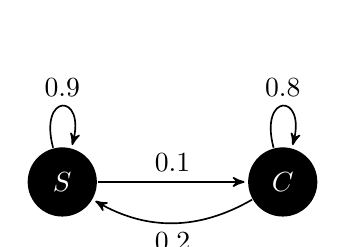
\begin{tikzpicture}[->,>=stealth',shorten >=1pt,auto,node distance=2.8cm,
  semithick]
  \tikzstyle{every state}=[fill=black,draw=none,text=white]

  \node[state]         (S)              {$S$};
  \node[state]         (C) [right of=S] {$C$};

  \path (S) edge [loop above] node {0.9} (S)
        (S) edge              node {0.1} (C)
        (C) edge [loop above] node {0.8} (C)
        (C) edge [bend left]  node {0.2} (S)
        ;
\end{tikzpicture}

\begin{align*}
  P = \begin{bmatrix}
       & S & C \\
   S   & 0.9 & 0.1\\
   C   & 0.2 & 0.8\\
  \end{bmatrix}
\end{align*}

\subsection{}
\begin{itemize}
  \item (i)
\begin{subequations}
  \begin{align}
    det(\lambda I - P) &= \begin{pmatrix}
    \lambda - 0.9 & -0.1\\
    -0.2 & \lambda - 0.8\\
  \end{pmatrix}\\
  &= \lambda^2 - \lambda 1.7 + 0.8\\
  \end{align}
\end{subequations}

Solving applying $ \frac{-b \pm \sqrt{b^2 - 4ac}}{2a}$ we get $\lambda_0 = 1$ and $\lambda_1 = 0.7$.

  \item (ii) Trace of A $ = \sum \text{diagonal } A = 0.9+0.8 = 1.7 = \lambda_0 + \lambda_1 = 1 + 0.7$.
  \item $det(P) = 0.9 * 0.8 - 0.1 * 0.2 = 0.7 = \prod_i \lambda_i = 1 * 0.7$

\end{itemize}

\subsection{}
For the case $\pi_s(n)$ starting in $n = 0$ with state $S$ which is Sunny we have
\begin{subequations}
  \begin{align}
    \pi_s(0) = a + b = ([1 0]P^0) = P_{ss}^0 = 1
  \end{align}
\end{subequations}

Therefore $a = 1$
\begin{subequations}
  \begin{align}
    \pi_s(1) = a + 0.7b = ([1 0]P^1) = P_{ss}^1 = 0.9
  \end{align}
\end{subequations}

Then,
\begin{subequations}
  \begin{align}
    0.9 &= 1 + 0.7b\\
    -0.7b &= 1 - 0.9\\
    b = -0.14
  \end{align}
\end{subequations}

Therefore $a = 1$ and $b = -0.14$.

Then $\pi_s(n) = 1 - 0.14 * 0.7^n, n \geq 0$

For the case cloudy $\pi_c(n)$ starting in $n = 0$ with state $S$ which is Sunny we have
\begin{subequations}
  \begin{align}
    \pi_c(0) = a + b = ([1 0]P^0) = P_{sc}^0 = 0
  \end{align}
\end{subequations}

Therefore $a + b = 0$
\begin{subequations}
  \begin{align}
    \pi_c(1) = a + 0.7b = ([1 0]P^1) = P_{sc}^1 = 0.1
  \end{align}
\end{subequations}

Then taking that $ a = -b$,
\begin{subequations}
  \begin{align}
    a &= -0.7b + 0.1\\
    a &= -b\\
    -b &= -0.7b + 0.1\\
    -b + 0.7b = 0.1\\
    -0.3 b = 0.1\\
    b = -0.33
  \end{align}
\end{subequations}

Therefore $a = 0.33$ and $b = -0.33$.

Then $\pi_s(n) = 0.33 - 0.33 * 0.7^n, n \geq 0$

\section{}

First we need to calculate the eigen values.
\begin{subequations}
  \begin{align}
    det(\lambda I - P) = \frac{-9\lambda^3+23\lambda^2-19\lambda+5}{9}
  \end{align}
\end{subequations}

And the roots are $\lambda_0 = 1, \lambda_1 = 0.55555, \lambda_2 = 0.99999$

\begin{subequations}
  \begin{align}
    \pi_2(n) &= a \lambda_0^n + b \lambda_1^n + c \lambda_2^n\\
    \pi_2(0) &= a + b + c = (\pi(0)P^0)_2 = 0\\
    \pi_2(1) &= a + 0.55 b + 0.99 c = (\pi(0)P^1)_2 = P_{12}^1 = \frac{15}{36}\\
    \pi_2(2) &= a + 0.55^2 b + 0.99^2 c = (\pi(0)P^2)_2 = P_{12}^2 = \frac{20}{36}\frac{15}{36} + \frac{15}{36} = \frac{35}{54}\\
  \end{align}
\end{subequations}
Solving the equation system we have that $a = \frac{25}{27}, b = -\frac{25}{27}, c = 0$.

Therefore, $\pi_2(n) = \frac{25}{27} - \frac{25}{27} * 0.55^n $. When $n \rightarrow \infty$ Probability is $\frac{25}{27}$ because second term tends to $0$.

\subsection{}
If $\pi_2(\infty) = \frac{25}{27} = 0.94$. In the previous exercise we have obtained the same number but with other fraction which is $\frac{15}{16}$ but the decimal number representation is the same.

\end{document}

